\chapter{Smart Contract Design and Implementation} \label{smart-contract-impl}

One of the major parts of this project's contributions is a smart contract with the necessary functionality to represent any given SmartFin financial contract definition (passed into the constructor), which is mainly interacted with through a web client. The syntax and semantics of SmartFin are described in chapter \ref{combinator-DSL}. This chapter will detail the design and implementation of this smart contract's general operation and ABI (the smart contract equivalent of an API), and evaluate to what level it is sufficient for its purpose of representing SmartFin contracts. \\

The elements covered in this chapter are displayed in a dependency graph in figure \ref{fig:smart-contract-block} . This chapter does not go into depth on the combinator implementation modules, which are instead described in chapter \ref{combinators-main}. \\

\begin{figure}[h]
    \centering
    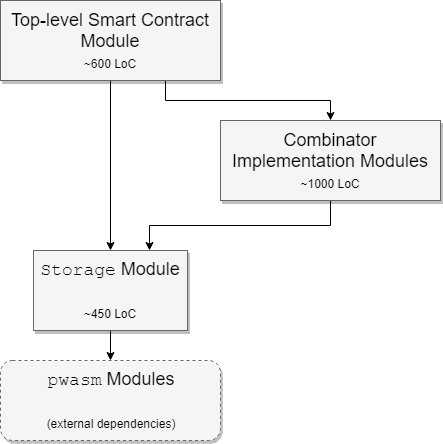
\includegraphics[width=0.5\textwidth]{smart-contract-block.png}
    \caption{A dependency graph of the modules used for the SmartFin smart contract, with their approximate \textit{Lines of Code} (not including tests). \texttt{pwasm} modules are external dependencies, described in section \ref{smart-contract-tech}. The combinator implementation modules are described in chapter \ref{combinators-main}.}
    \label{fig:smart-contract-block}
\end{figure}


\section{Requirements} \label{contract-requirements}

In order to ensure that the smart contract accurately and correctly represents SmartFin contracts, a set of requirements has been devised. These requirements form the motivation behind specific design and implementation choices made during the creation of the smart contract. \\

The SmartFin contracts that can be represented by the smart contract consist of an agreement between two parties (the \textit{holder} and \textit{counter-party}) with regards to payments between these parties. As such, the smart contract must hold the definitions of both the holder and counter-party, and allow the two parties to exchange funds through the contract. \\

The holder should have the ability to acquire the contract (just as they would be able to sign a traditional financial contract), and this should result in the evaluation of payments to be made between the two parties with respect to the acquisition time. \\

The smart contract should also be able to represent the behaviour/state of the combinators defined in section \ref{DSL-design}. The evaluation of the payments between the two parties should respect the semantics of these combinators. \\

Certain values in the SmartFin contract may be unknown until a later point (for example, observables in a \texttt{scale} combinator), and so the smart contract requires some way of obtaining these values. The holder may also be able to choose certain options on the SmartFin contract (for example, choosing a branch of an \texttt{or} combinator), and the smart contract should also facilitate this. \\

The evaluation of payments between the two parties may change over time. For example, the SmartFin contract \texttt{get truncate (01/01/2020 12:00) one} requires a payment to occur from the counter-party to the holder at noon on the 1st of January 2020. Before this time, no payments should occur. This means that the smart contract must be able to keep track of the state of the SmartFin contract's obligations over time. \\

All of these are specific requirements that are required for the smart contract to accurately represent any given SmartFin contract. These have been taken into consideration during the design and implementation of the smart contract, informing the final product.


\section{Design} \label{contract-design}

The overall design of the smart contract is fairly simple, albeit with several caveats. From a very high level, the smart contract consists of a class with an ABI, several state variables, and a tree of \texttt{ContractCombinator} objects. The behaviour of the SmartFin combinators is implemented by the \texttt{ContractCombinator} objects, the entire tree represent the SmartFin contract definition, and the rest of the smart contract effectively informs the way that it operates as a whole. See section \ref{combinators-design} for details on the representation of individual SmartFin combinators.


\subsection{High Level Design Challenges}

In an ideal world, the smart contract would track payments over time and exchange funds between the required parties immediately, as one might expect from a web-service or similar. Unfortunately, the smart contract runs on a blockchain, and as such there are several restrictions which affect its ability to operate as required. These inform the high-level design of the smart contract.

\subsubsection{Payment Evaluation}

It is not possible to schedule callbacks on a blockchain without relying on external tools, as this would jeopardise determinism, and it would require a miner to run the code at a specific time. As such, the smart contract is only able to perform execution when called into from a user. \\

Certain SmartFin contracts require payments to occur at specific times; for example, the contract \texttt{get truncate \textit{t} one} requires the counter-party to pay the holder 1 Wei at time \textit{t}. Unfortunately, smart contracts are unable to make payments at specific times, as this would require scheduled callbacks to be possible. \\

In order to represent time-respective payments, the implemented smart contract allows payments to be fulfilled retroactively. In essence, the smart contract does not perform payments at specific times, but instead keeps track of important times - typically combinators' acquisition times - and evaluates which payments should have occurred since that time after the fact. \\

To facilitate this, payments between the two parties are represented as a balance, changing when either party stakes/withdraws funds to/from the contract, or when payments are evaluated. In order to evaluate the payments which should have occurred by the current point in time, the smart contract has an \texttt{update} method which calculates the new balance between the holder and counter-party, resulting from any payments defined by the SmartFin contract definition between the last \texttt{update} call and the current block-time. For example, when the holder acquires the contract \texttt{get truncate \textit{t} one} before time \texttt{\textit{t}}, their balance does not change, and their balance does not change when \texttt{\textit{t}} passes either. Only once the contract is updated \textit{after} time \texttt{\textit{t}} does this balance change. This is depicted in figure \ref{fig:contract-update}. \\

\begin{figure}[h]
    \centering
    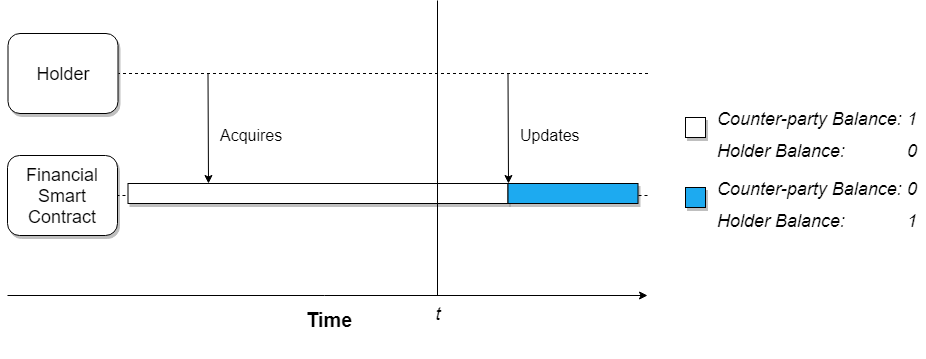
\includegraphics[width=\textwidth]{contract-update-diagram.png}
    \caption{A diagram depicting the balance of the holder and counter-party over time for the financial smart contract representing the SmartFin contract \texttt{get truncate \textit{t} one}.}
    \label{fig:contract-update}
\end{figure}

\subsubsection{Observable Evaluation}

Similar to the evaluation of payments, another factor in SmartFin contracts which changes over time is observables. These are objective, potentially time-varying quantities. An example of an observable which does not vary over time would be the number 5, whereas an example of an observable which does vary over time is the average temperature of London in Celsius. Both are objective, but one takes different values depending on what time you sample it. \\

Unfortunately, this poses a couple of problems for the smart contract. As mentioned earlier, smart contracts cannot schedule callbacks at specific times, and so finding the value of an observable at a specific time is not a simple task. There is also the issue that smart contracts are unable to access information which is not stored on the blockchain, which means that sampling observable values from websites or other off-chain sources is not possible. \\

These two restrictions effectively rule-out the possibility of the  smart contract obtaining the value of a time-varying observable without external interaction from the user. To work around this issue, when a SmartFin contract relies on an observable the author must define an \textit{arbiter} for its value. This arbiter is an address which can provide the observable's acquisition-time-value to the contract, effectively acting as a trusted source of information. \\

When an observable's value is unknown while the smart contract is being updated, the sub-contract relying on the observable will not be updated until the value is provided. After its provision, the sub-contract can be updated, thus allowing retroactive provision of observable values. For example, take the financial smart contract representing the SmartFin contract \texttt{scale \textit{x} <arbiter address> one}; when acquiring the contract before the observable's value is set, the balance does not change. Once the arbiter sets the value of the observable to 1, and then the financial smart contract is updated, the balance changes. This is depicted in figure \ref{fig:contract-scale-update}. \\

\begin{figure}[h]
    \centering
    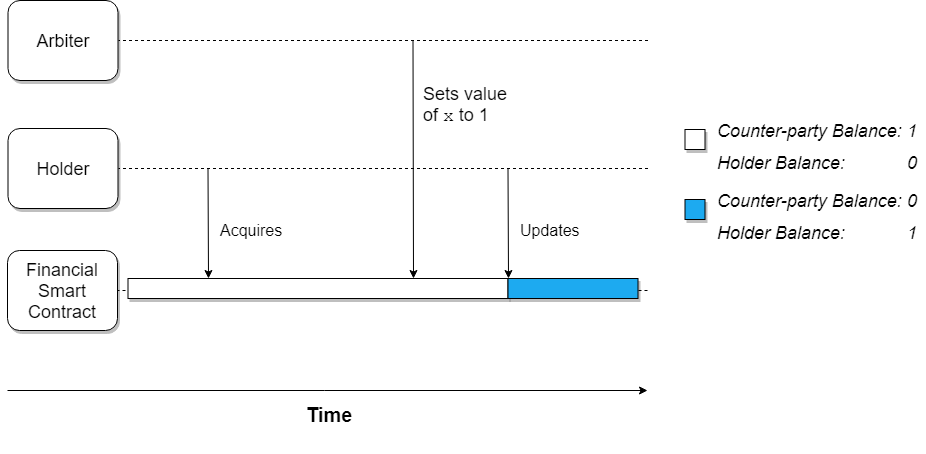
\includegraphics[width=\textwidth]{contract-scale-diagram.png}
    \caption{A diagram depicting the balance of the holder and counter-party over time for the financial smart contract representing the SmartFin contract \texttt{scale <observable name> <arbiter address> one}.}
    \label{fig:contract-scale-update}
\end{figure}

\subsubsection{Exchanging of Funds}

As you have hopefully noticed by now, smart contracts deal heavily with the exchanging of funds. Regular financial contracts are typically binding, requiring one party to pay the other party or risk legal action. Smart contracts are a little different; they have no way to ensure that one user will pay another user, but instead act as a separate entity which processes payments from both both parties. \\

A disadvantage of this is that the implemented smart contract is unable to force one party to pay the other party. It can maintain a balance between the two parties, indicating when one party \textit{should} pay the other, but it has no means to enforce this payment. In order to somewhat circumvent this issue, the smart contract allows users to stake Ether in the contract at any time (increasing their balance), and to withdraw Ether under certain conditions. In order to withdraw an amount of Ether: \\

\begin{itemize}
    \item The user must have enough Ether in their balance.
    \item The smart contract must have enough total balance.
    \item The user's balance must be larger than withdrawal gas fees (where gas fees apply). \\
\end{itemize}

By allowing the parties to stake Ether in the smart contract beforehand, the smart contract is able to make any required payments without immediate action from the paying party as long as it has enough funds. Incidentally, this is another reason that retroactive payments are appropriate, as there is no guarantee that the smart contract will actually have the funds to pay a party when a payment should occur. \\

Unfortunately, it is still impossible for the smart contract to solve the issue of binding a party to payment. As such, if one party decides not to pay, they can simply refuse to stake any Ether and thus the smart contract will have no funds to pay the other party. There were a few possible solutions (or at least mitigations) to this issue. \\

Restricting withdrawal from the smart contract until its conclusion would prevent parties from withdrawing before they have to make a payment. Unfortunately, it would also lower the value obtained through the contract, as funds locked in the contract's balance could instead be earning money through investment. Another potential solution could be to prevent contract acquisition until sufficient funds have been staked in the smart contract, but this has a similar issue that funds staked in a smart contract would be better served elsewhere. \\

The best solution to this issue is to use financial smart contracts alongside a legally-binding contract requiring a party to stake funds when required. For now, we assume that each party is bound to make payments to the smart contract in an honest way, as it seems that this is not something that can be solved in a satisfactory manner through the smart contract itself.


\subsection{Financial Smart Contract ABI} \label{smart-contract-ABI}

The smart contract has a set of functions which can be called by the web client, allowing it to interact with and monitor the contract. This ABI is informed by the requirements of the smart contract, and any caveats encountered due to its nature as a smart contract. The behaviour of many of these functions is determined by the composition of combinators used to write the SmartFin contract passed-in to the smart contract's constructor. The full financial smart contract ABI is listed in appendix \ref{appx:ABI}.


\subsubsection{Constructor}

The constructor of the smart contract is responsible for initialising the smart contract object, and as such it requires all information relevant to the initial state of the SmartFin contract. The constructor takes the following parameters: \\

\begin{itemize}
    \item The SmartFin contract definition.
    \item The address of the contract holder.
    \item Whether or not the contract should allocate gas fees upon withdrawal (as private blockchains do not always require gas fees).
\end{itemize}


\subsubsection{Pure Functions}

The smart contract defines several functions which return the value of state variables (i.e. \textit{getter} functions). This enables the web client to display the current state of the contract. As these are \textit{pure} functions, they do not cost any gas to call, and thus the web client may update its view of the smart contract as often as required at no cost. These functions consist of the following: \\

\begin{itemize}
    \item \texttt{get\_holder}: Returns the address of the contract's holder.
    \item \texttt{get\_counter\_party}: Returns the address of the contract's counter-party.
    \item \texttt{get\_contract\_definition}: Returns the SmartFin contract definition.
    \item \texttt{get\_balance}: Returns the balance of one of the parties (in Wei).
    \item \texttt{get\_concluded}: Returns whether or not the smart contract has concluded execution (i.e. no more updates are required).
    \item \texttt{get\_use\_gas}: Returns whether or not the smart contract allocates gas fees upon withdrawal.
    \item \texttt{get\_last\_updated}: Returns the block-time that the last call to the \texttt{update} function occurred at.
    \item \texttt{get\_acquisition\_times}: Returns a list of the acquisition times of the contract and its sub-contracts.
    \item \texttt{get\_or\_choices}: Returns a list of choices which have been made for \texttt{or} combinators.
    \item \texttt{get\_obs\_entries}: Returns a set of observables, including their names, values, and arbiter addresses.
\end{itemize}

\subsubsection{Setting Values}

The smart contract has several values which rely on user input to evaluate. One such combinator is the \texttt{or} combinator, which allows the holder to acquire either of its two sub-contracts at the time of acquisition. The holder is able to call the function \texttt{set\_or\_choice} at any time, to inform the smart contract of which sub-contract the holder should acquire for a given \texttt{or} combinator. An \texttt{or} choice cannot be changed after it has been made, to prevent inconsistency across multiple updates. \\

Another combinator which requires user input is the \texttt{scale} combinator. For each \texttt{scale} combinator's observable, if said observable is not a constant then it will require an arbiter to provide its value. The arbiter can call the \texttt{set\_obs\_value} function to set the value of an observable at any time, once per observable.

\subsubsection{Acquisition}

The holder must have the ability to acquire the smart contract, just as a prospective holder would be able to acquire a traditional financial contract by signing it. As such, the smart contract's ABI contains an \texttt{acquire} method, callable by the holder. This method updates the contract state to store the time of acquisition. \\

Besides the top-level contract, \texttt{anytime} combinators can also be acquired at certain times during the smart contract's lifetime. As such, there is also an \texttt{acquire\_anytime\_sub\_contract} method; if the acquisition is valid (i.e. the \texttt{anytime} combinator's parent is acquired, and the combinator is not expired), then the smart contract will update its state to reflect that the sub-contract has been acquired.

\subsubsection{Update}

Due to the nature of the blockchain, the smart contract cannot keep itself up-to-date without external action. The \texttt{update} function causes the smart contract to evaluate the difference in balance between the current \texttt{update} call and the last \texttt{update} call, retroactively evaluating payments. The \texttt{update} function can be called from any address, as the update operation is handled entirely by the smart contract with no external inputs.

\subsubsection{Payment and Withdrawal}

The smart contract allows either party to stake Ether, to facilitate payments between them. The \texttt{stake} method is a \textit{payable} function (i.e. it can receive Ether), which increases the balance of the party that called it by the amount of Ether received. \\

The smart contract also allows either party to withdraw Ether, assuming the balances allow it. To do this, the \texttt{withdraw} method takes an amount and sends the requested amount of Ether to the calling party, reducing their balance by the withdrawn amount. Gas fees (when enabled) are taken out of the party's balance on top of the withdrawal, or out of the withdrawal amount if the balance hits 0. Besides the two involved parties, no addresses can stake or withdraw Ether - it would be unclear who to allocate staked Ether to, and only the respective party should be able to withdraw from their balance.


\section{Implementation}

\subsection{Technologies} \label{smart-contract-tech}

In order to implement the smart contract, there were several choices to make with regards to which technologies would be employed. As discussed in section \ref{DSL-implementation-technologies}, there are many possible tools with which to implement a smart contract. \\

The final method that was decided upon for implementing the smart contract was the use of Rust\cite{rust} with \textit{pwasm} modules/tools provided by Parity Technologies\cite{parity-technologies} for compilation to WebAssembly. The final WebAssembly contract is compatible with private blockchains run from Parity's own Ethereum client, as well as with the Kovan test network and other wasm-compatible Ethereum clients\cite{pwasm-tut-node}. \\

The pwasm modules provide various tools for developing smart contracts in Rust, as discussed in section\ref{dev-tools}. The main tools which were made use of in the smart contract implementation were: \\

\begin{itemize}
    \item \texttt{pwasm-std}: A module re-implementing useful pwasm-compatible functionality from the Rust standard library (which is not compatible with these pwasm modules).
    \item \texttt{pwasm-ethereum}: A module providing access to information and functionality from the blockchain, including the current block-time, the address of the caller, writing to or reading from smart contract storage, and more.
    \item \texttt{pwasm-abi} and \texttt{pwasm-abi-derive}: Modules which enable the conversion of a Rust trait into a smart contract ABI definition.
    \item \texttt{pwasm-test}: A unit testing framework for smart contracts written in Rust. \\
\end{itemize}

Unfortunately, due to the pwasm modules' incompatibility with the Rust standard library, it was impossible to use most external modules for the Rust smart contract. The smart contract implementation was possible without requiring any more external modules, but certain problems like serialization of structs could be solved much more easily using external libraries if it were possible. \\

In order to build the Rust smart contract, \textit{Cargo}\cite{cargo} (the Rust package manager) was used. Parity also provides a build tool for building wasm contracts with Cargo, \textit{wasm-build}\cite{pwasm-build-tools}. \textit{Web3.js}\cite{web3-intro} was also used to deploy smart contracts to the blockchain, and interact with them (for testing purposes). This was managed with \textit{yarn}\cite{yarn}, a package manager for JavaScript.


\subsection{Smart Contracts in Rust}

Rust smart contracts implemented using the pwasm modules must be defined in a particular manner. Firstly, the Rust program must have a few things implemented in the main module of the application (typically written in \texttt{lib.rs} for a Rust program), including a smart contract ABI, a smart contract struct, and a \texttt{call} and \texttt{deploy} function. \\

The smart contract's ABI is defined through a trait (a set of several methods) with annotations. Pure methods (i.e. those that do not alter smart contract state) are denoted by the \texttt{constant} annotation, and payable methods (i.e. those that can receive Ether) have the \texttt{payable} annotation. There must also be a \texttt{constructor} method implemented, which initialises the smart contract struct/state on deployment. This trait is then used to generate the smart contract ABI, as well as to generate an \textit{endpoint} which delegates method calls to the smart contract struct. Only certain types are able to be sent/received via a pwasm smart contract's ABI, including integer types, vectors, addresses, booleans, and a few more binary data types. \\

A smart contract struct must also be implemented. This is a data type which must implement the ABI trait. Every time the smart contract is called into, a new instance of the smart contract struct is constructed. This means that member variables on the struct will be reset every time that the smart contract is called into. In order to store persistent state across smart contract calls, the smart contract storage must be manually written to/read from (using methods provided by \texttt{pwasm-ethereum}). \\

Alongside the ABI and smart contract struct, public static \texttt{call} and \texttt{deploy} functions must be implemented. The \texttt{call} function will initialise the smart contract struct, and an \textit{endpoint} which delegates method calls based on the ABI, and handles smart contract calls by providing the call inputs (method name, parameters, etc.) to the endpoint. The \texttt{deploy} function is similar, but is called when the smart contract is first deployed to forward the inputs for the constructor call to an initialised endpoint.


\subsection{ABI Methods}

\subsubsection{Constructor}

The constructor is called when the smart contract is initially deployed, and is responsible for setting up the initial state. Firstly, the validity of the constructor arguments is checked, throwing an error if any invalid arguments are passed; throwing an error will cause smart contract methods to cease execution and roll-back state changes. After checking the arguments, the constructor writes several values to storage, including the holder and counter-party addresses, the holder and counter-party balances, whether or not the contract uses gas, the last-updated time, and the contract definition. \\

The contract definition is passed to the constructor as the type \texttt{Vec<i64>}, i.e. a vector of signed 64-bit integers. This is necessary as Rust smart contracts written with pwasm modules cannot send/receive strings over the ABI, and thus the contract definition must be provided in a serialized form. The serialized form of SmartFin simply involves representing the SmartFin contract as an array of integers. Each combinator is represented by an integer (0 to 9), times are represented as UNIX Epoch times, integer values are unchanged, names are represented by arrays of character codes, and addresses are represented by an array of four integers. The contract definition is deserialized recursively into a set of \texttt{ContractCombinator} objects, representing the SmartFin combinators. For more information on how the combinators are represented in the Rust smart contract, see chapter \ref{combinators-main}.


\subsubsection{Pure Methods} \label{ABI-pure}

The pure ABI methods (i.e. getters) are generally quite straightforward; \texttt{get\_holder}, \texttt{get\-\_counter\_party}, \texttt{get\_contract\_definition}, \texttt{get\_balance}, \texttt{get\_use\_gas}, \texttt{get\_last\_updated}, and \texttt{get\_acquisition\_times} all read the required data from storage and return it in a trivial manner. \\

\texttt{get\_concluded} returns \texttt{true} if the contract will no longer change state over time, i.e. all responsibilities are fulfilled. This is true if the contract has been acquired and the combinators have been fully updated to their final state, or if the contract has expired before acquisition. \\

\texttt{get\_or\_choices} reads the set of choices for \texttt{or} combinators from storage, and then serializes this into a vector of bytes. \texttt{1} represents the first sub-contract, \texttt{0} the second, and \texttt{2} means that no choice has been made yet. \\

\texttt{get\_obs\_entries} constructs and returns the set of observable entries for the contract from storage. This consists of a vector of observables, with their arbiter address, value, and name (all serialized as several signed 64-bit integers).


\subsubsection{Sub-contract Acquisition and Setters}

The functions setting \texttt{or} combinator choices, observable values, and acquiring \texttt{anytime} sub-cont\-racts are also quite straightforward. The \texttt{or} choices, observable values, and \texttt{anytime} acquisition times are all stored as vectors in the smart contract storage. In order to update any of these values, the relevant element in the vector is written to directly through a storage object, described in section \ref{storage}. Acquiring an \texttt{anytime} combinator's sub-contract will also update the contract, with a call to \texttt{update}.


\subsubsection{Acquire}

The \texttt{acquire} method first reads and deserializes a combinator object from storage, which implements a combinator contract's behaviour. If the caller is the holder and the combinator hasn't been acquired already, the method calls an \texttt{acquire} method on the contract combinators, passing down a reference to the storage object. For more information on the combinator objects' \texttt{acquire} methods, see section \ref{combinator-implementation}. The combinator object is then serialized and re-written into storage.


\subsubsection{Update}

The \texttt{update} method first checks if the contract has concluded. If so, then updating the contract will have no effect no matter what happens, so the contract throws an error. After this, the combinator object is read from storage and deserialized, as in the \texttt{acquire} method. The storage object is passed to the \texttt{update} method on the combinator object, which is also described in section \ref{combinator-implementation}. The combinators are then serialized and written back to storage. \\

After updating the combinators, the new balances of the holder and counter-party are written to storage. These are calculated using a \texttt{safe\_add} method, which checks for integer overflow. Rust should throw an error automatically if it occurs, but extra precaution is taken due to the severity of overflow errors with balances in smart contracts.


\subsubsection{Stake}

The \texttt{stake} method is a \texttt{payable} function, to which Ether is paid upon calling. The \texttt{pwasm-ethereum} function to obtain the value of a transaction returns a \texttt{U256}, i.e. an unsigned 256-bit integer. Balances are stored in the smart contract storage as signed 64-bit integers, as they are easier to work with being Rust primitive types. Because of this, the \texttt{stake} method must first check that the value provided can be converted into a signed 64-bit integer, or an error is thrown. \\

After checking this, the method checks whether the caller is the holder or the counter-party - an error is thrown otherwise. The method then safely adds the value of the method call transaction to the balance of the relevant party, and writes the new balance to storage.


\subsubsection{Withdraw}

The \texttt{withdraw} method allows a user to withdraw funds from the contract by initiating a transfer of Ether from the smart contract to the caller. First, the method checks which address to withdraw Ether from. If the caller is not one of the holder or the counter-party, then an error is thrown. \\

The method calculates how much Ether to send by comparing the amount requested to the balance of the relevant party, the total contract funds, and the gas cost. If the contract allocates gas fees upon withdrawals, then 2300 Wei in gas fees is added to the withdrawal amount. If either of the total funds of the contract or the party's balance are smaller than the gas cost, then an error is thrown. The withdrawal amount (including gas fees) is clamped to the minimum of the party's balance and the total funds. If the final amount is 0 or less, then an error is thrown. \\

After the viable withdrawal amount is calculated, the relevant balance is updated, and then the method creates a transaction from the smart contract to the caller address. If the transaction fails then the relevant balance is rolled back to its original amount, and an error is thrown.


\subsection{Storage} \label{storage}

Besides the ABI methods and combinator behaviours, the other main functionality that the smart contract implemented was storage. State - such as the holder address, acquisition times, or the combinator objects - must be stored in smart contract storage in order to remain persistently across multiple smart contract method calls. In order to do this, the \texttt{Storage} module was implemented to handle the storage of various data types.


\subsubsection{Memory Layout of Smart Contract Storage}

Smart contract storage is addressed using 256-bit integers (of the type \texttt{H256}), and each slot in storage can store 256 bytes of information in the form of an array of 32 unsigned 8-bit integers. In order to separate storage into different spaces, the most-significant byte of each memory address is treated as a "namespace" byte by the smart contract. The hexadecimal addresses \texttt{0x0000...00} to \texttt{0x00FF...FF} span the first memory namespace, \texttt{0x0100...00} to \texttt{0x01FF...FF} span the second memory namespace, etc. As such, if a function is writing to storage sequentially and reaches the end of a namespace, by incrementing the most-significant byte, then an error must be thrown.


\subsubsection{Storage Module Design}

The \texttt{Storage} module contains definitions for a \texttt{Storage} struct and several traits which include methods to read from/write to smart contract storage. The reason that a struct is used instead of static methods is that data read from/written to smart contract storage is cached in the Storage object, and so only one read to smart contract storage must occur for each object being read per ABI method call. The cache is destroyed between ABI method calls as the smart contract struct is destroyed after the ABI call finishes and the smart contract is exited. Cached reads/writes are stored in a vector of \texttt{Entry} struct instances, which contain the storage address and a value. \\

There are also three generic traits which are used for storage; the \texttt{StoresFixed<T>} trait indicates that the implementing struct can store a value of the type \texttt{T} in memory, and that the size of any values of this type is constant. The size restriction is helpful as it ensures that values can be stored sequentially in smart contract storage without changing in size and overwriting each other, or leaving empty space between elements. The trait defines methods for reading/writing a value, and a static \texttt{size} method. \\

The second generic trait used for storage is \texttt{StoresFixedVec<T>}, which indicates that the implementing struct can store an object of the type \texttt{Vec<T>} in memory, where elements of type \texttt{T} have a known fixed size. This trait allows reading/writing the whole vector to storage with linear time complexity, as well as getting the length, reading/writing individual elements, and pushing elements to the end of the array with constant time complexity. \\

The third trait used for storage is \texttt{StoresVariable<T>}, which indicates that the indicating struct can store an object of the type \texttt{T} in memory, but its size is unknown and/or variable. This trait allows writing or reading of whole objects of type \texttt{T} with linear time complexity. \\

All write and read methods return a key along with any other value. This key represents the last storage address used in the method. For example, if a vector is stored at address 2 and takes up 6 slots, the read/write methods will return address 7. This enables sequential writing of values in memory, especially useful when those values have variable size.


\subsubsection{Storage Method Implementation}

Besides several implementations of the traits mentioned above, the \texttt{Storage} struct also has method implementations for several of its own helper methods, for converting values between types. The \texttt{Storage} struct also has a constructor which will initialise the storage cached vector to empty. \\

Only one type can be read from/written to smart contract storage using the \texttt{pwasm-ethereum} \texttt{read}/\texttt{write} functions, an array of 32 unsigned 8-bit integers (i.e. \texttt{[u8; 32]}). Several methods on the \texttt{Storage} struct implement conversion of other types to/from this type. The \texttt{from\_address} method converts an address into an \texttt{H256} data type using the \texttt{H256::from} function, which can be converted directly into a \texttt{[u8; 32]} object. The method \texttt{to\_address} converts similarly in the opposite direction. \\

The \texttt{from\_bool} method converts a boolean value into \texttt{[u8; 32]}. In the case of \texttt{false}, the function returns a \texttt{[u8; 32]} array with all elements set to 0, otherwise an element is set to 1. The \texttt{to\_bool} method can thus return whether or not the given \texttt{[u8; 32]} is not equal to \texttt{H256::zero()}. \\

The last pair of conversion functions that the \texttt{Storage} struct implements is \texttt{to\_i64} and \texttt{from\_i64}. As the \texttt{pwasm-std} module implements functions \texttt{read\_u64} and \texttt{write\_u64}, which convert an unsigned 64-bit integer (i.e. \texttt{u64}) to/from \texttt{[u8; 32]}, the \texttt{i64} conversion methods use this method and convert between \texttt{i64} and \texttt{u64}. \\

To convert from a \texttt{u64} to an \texttt{i64}, first the value of the \texttt{u64} is checked. If the \texttt{u64} value is less than $2^{63}$, then it can be directly converted to an \texttt{i64}. This is because binary representation of an integer in the range of $0$ to $2^{63} - 1$ is equivalent for both types. For an n-bit unsigned integer, the value can be calculated as $2^0 \cdot b_0 + 2^1 \cdot b_1... + 2^{n-1} \cdot b_{n-1} + 2^n \cdot b_n$, where $b_i$ is the value of the \texttt{i}'th least significant bit. For an n-bit two's complement integer, the equivalent expression would be $2^0 \cdot b_0 + 2^1 \cdot b_1... + 2^{n-1} \cdot b_{n-1} - 2^n \cdot b_n$. As such, as long as the most-significant bit is 0, then the decimal value of an \texttt{i64} and a \texttt{u64} with the same binary representation is equal. If the \texttt{u64}'s most significant bit is 1, then we can convert to two's complement by subtracting $2^{64}$. This must be done in a slightly roundabout manner in Rust, by subtracting $2^{63}$ to convert the \texttt{u64} into the range of an \texttt{i64}, and then subtracting $2^{62}$ twice (as $2^{63}$ cannot be represented as an \texttt{i64}). The reverse conversion from \texttt{i64} to \texttt{u64} is similar, requiring $2^{64}$ to be added rather than subtracted.


\subsubsection{Static Storage Module Functions}

The \texttt{Storage} module also provides several static functions. Functions for converting between an \texttt{Address} and an array of four \texttt{i64}s are provided. To convert from an \texttt{Address} to four \texttt{i64} values, \texttt{address\_to\_i64} converts the address to a storable \texttt{[u8; 32]} array using \texttt{Storage::from\_address}. This array is split into four separate 32-byte storable values, where the first 8 bytes of each is a quarter of the storable value, and the rest are 0. These can be converted to an \texttt{i64} using \texttt{Storage::from\_i64}. The function \texttt{i64\_to\_address} works similarly in the opposite direction. \\

The \texttt{Storage} module also provides a private function \texttt{add\_to\_key}. This function takes a storage key (as an \texttt{H256}) and an unsigned 64-bit integer value, and increments the address by the value. This is done by repeatedly incrementing the least-significant bit of the address, and decrementing the value, until the value hits zero. If the least-significant bit overflows, then it is set to 0 and the next least-significant bit is incremented. This is repeated if the next least-significant bit is incremented. If the second most-significant byte overflows, than an error is thrown as this would violate the separation of memory namespaces mentioned in the \textit{Memory Layout of Smart Contract Storage} segment of this section.


\subsubsection{\texttt{StoresFixed} Implementation for \texttt{[u8; 32]}}

For the \texttt{write} method implementation, the storable array is first written into the smart contract storage using \texttt{pwasm-ethereum}'s \texttt{write} method. After this, the \texttt{Storage} struct's cache is checked for the presence of the given key. If the key is present, the value is updated to the new value provided, otherwise it is added to the table. For the \texttt{read} implementation, the cache is checked for the presence of the given key. If this hits, then the corresponding value is returned, otherwise it is read from smart contract storage and written into the cache before being returned. The storage address returned from both of these methods, representing the last-used address in writing the given object to storage, is the same as the key passed in - this is because a \texttt{[u8; 32]} value can be stored in one storage slot. \\

\subsubsection{\texttt{StoresFixed} Implementation for Primitive Types and Address}

As mentioned earlier, the \texttt{Storage} struct implements several conversion methods between primitive types (\texttt{u32}, \texttt{i64}, \texttt{bool}) or \texttt{Address} values and storable values (\texttt{[u8;32]}). Leveraging this, the \texttt{StoresFixed} implementations for these types simply convert the values into a \texttt{[u8; 32]} value and call into the \texttt{StoresFixed<[u8; 32]>} implementations.


\subsubsection{\texttt{StoresFixed} Implementation for \texttt{Option<T>}}

In order to store values of type \texttt{Option<T>} (which take the value \texttt{None} or \texttt{Some(v: T)}), we must be able to store values of type \texttt{T} and a value to indicate whether or not the object has a concrete value. The \texttt{write} method for \texttt{Option<T>} will pattern match the given value, and write a boolean \texttt{true} or \texttt{false} depending on whether a concrete value exists. If one exists, it is written to the next slot in storage; if not, nothing is written to the next slot in storage. Either way, the last-used key returned is the passed-in key plus the size of \texttt{T} in storage, in order to reserve a second slot in storage regardless of whether a value was written (or else the storage size of \texttt{Option<T>} would not be fixed). The \texttt{read} method simply checks if a value is stored or not, then reads and returns \texttt{Some(value)} or \texttt{None}.


\subsubsection{\texttt{StoresFixedVec} Implementation}

Vectors are stored in smart contract storage sequentially, with the first storage slot containing the number of elements in the vector, and the following slots containing values written using the \texttt{StoresFixed<T>} implementation. Vectors are always written in their own memory namespace - i.e. their most-significant byte is unique - to prevent a change in size from overwriting adjacent values in storage. \\

The \texttt{write\_vec} implementation gets the length of the given vector and writes that to the first storage slot. After this, the vector is processed to write each element into storage sequentially. The last-used key is kept track of throughout this process, and returned after the whole vector is stored. The \texttt{read\_vec} implementation is similar, first reading the vector length and then reading the elements sequentially from storage into a new vector, returning the last-used key. The \texttt{length} method simply reads the length from the first storage slot of the vector, and \texttt{set}/\texttt{get}/\texttt{push} which deal with individual vector elements will find the address of the required index by calculating the starting address plus the size of storing values of type \texttt{T} multiplied by the index.


\subsubsection{\texttt{StoresFixed} Implementation for Tuples}

\texttt{StoresFixed} is implemented for tuples with two and three elements, where an implementation of \texttt{StoresFixed} exists for all element types. This allows the smart contract to store small generic sets of data without implementing a specific struct, like an observable's arbiter, name, and value. Tuples are stored sequentially in memory, which is trivial using the \texttt{write}/\texttt{read} implementations of the tuple element types.


\subsubsection{\texttt{StoresVariable} Implementation for Vectors and Observable Names}

When the smart contract is constructed, a set of serialized observable names is generated from the given combinator contract. These are represented by a vector of integers per observable name; to store these names, a vector of vectors must be stored. As a vector of integers can grow and shrink, a \texttt{StoresFixedVec<Vec<T>{}>} implementation cannot be used. As such, \texttt{StoresVariable} exists to allow writing/reading variable-sized objects to and from storage in their entirety. \texttt{StoresVariable} is implemented for \texttt{Vec<T>} where \texttt{StoresVariable<T>} is implemented, and for \texttt{ObsName} - a struct containing the serialized observable name vector. The implementations are similar to the \texttt{StoresFixedVec<T>{}>} implementation, without the element-wise methods.


\section{Evaluation} \label{DSL-impl-evaluation}

In order to evaluate the design of the smart contract (minus combinator implementations), there are a couple of methods that can be employed. Qualitative analysis of the design of the smart contract's ABI can evaluate how well the smart contract fulfils the requirements laid out in section \ref{contract-requirements}. Qualitative analysis of the \texttt{Storage} module can also be employed to evaluate its design. Automated tests have also been used to ensure that the smart contract operates correctly, as described in section \ref{contract-design}, and that the \texttt{Storage} module operates as expected.

\subsection{Design of the Smart Contract's ABI}

To evaluate the smart contract's ABI, it can be compared to the requirements laid out in section \ref{contract-requirements}. The first requirement described the requirement that a financial smart contract should represent an agreement between a \textit{holder} and a \textit{counter-party}, and should allow the two parties to exchange funds. This is implemented in the contract by storing the holder and counter-party's addresses, and the staking and withdrawal of funds from the smart contract allows an indirect exchange of funds between the two parties.

Unfortunately, the smart contract does not facilitate direct payments between the two parties, but this would be impossible as a smart contract cannot initiate a transaction with another user's funds. Another issue with this implementation is that payments do not occur in real time, but instead retroactively through the \texttt{withdraw} method. Due to the lack of scheduled callbacks, and the requirement that funds are staked before being sent by a transaction, this would also not be possible. Retroactive payments are the next best option, and are not too dissimilar to the way that some financial contracts would handle transactions, e.g. via an escrow mechanism. \\

The second requirement was that the holder should be able to \textit{acquire} the contract, which should result in the evaluation of payments between the holder and the counter-party, with respect to acquisition time. This is implemented through the \texttt{acquire} method on the smart contract, allowing the holder to acquire it at any point in time, and evaluating payments required between the two parties - represented by a balance for each party. Assuming that the evaluation of these payments is correct (discussed in section \ref{contract-testing}), then this requirement is aptly fulfilled. \\

The third requirement, requiring the evaluation of payments to respect the given financial combinator contract's expected behaviour, is handled by the implementations of the combinators. This is detailed in section \ref{combinators-main}. \\

The fourth requirement requires the setting of observable values and \texttt{or} combinator branch choices to be possible. The setting of observable values is implemented through the \texttt{set\_obs\_value} method on the smart contract's ABI, which allows pre-defined arbiters to provide the values of observables. Ideally, the observables' values could be obtained automatically by the smart contract, but due to the lack of scheduled callbacks or off-chain interaction this is not possible. The implemented solution is the next best option.

The choosing of \texttt{or} combinator sub-contracts is implemented via the \texttt{set\_or\_choice} method on the ABI, allowing the holder to choose which sub-contract to acquire when the given \texttt{or} combinator is acquired. This works similarly to how a real financial contract works, where the holder must choose the sub-contract by making a choice manually, and so the requirement is fully met. \\

The final requirement described earlier is for the smart contract to keep track of the evaluation of payments over time. This is handled by keeping track of the balance of the holder and counter-party, and by updating it retroactively through calls to the \texttt{update} method in the smart contract's ABI. This method evaluates the difference in balance due to payments occurring since the last \texttt{update} call, thus keeping track of payments over time. Assuming that evaluation of payments is correct, as evaluated in section \ref{contract-testing}, then this method of keeping track of payments over time is sufficient to fulfil this requirement. \\

Based on these requirements - while there are some issues due to the lack of scheduled callbacks, off-chain interactions, and so-on - the final implementation is still sufficient to represent a traditional financial contract as a smart contract with similar behaviour. \\

Besides these requirements, there is one issue which plagues the smart contract's ABI: serialization. Most methods involve some level of serialization, with serialized arguments or return types. The reason that this is an issue is that it causes the smart contract to be very difficult to interact with from a command-line. Unfortunately, this issue is somewhat unavoidable due to the inability to send strings over a smart contract ABI implemented with \texttt{pwasm-abi}; implementing the smart contract in another language, like Solidity, may have avoided this however. The issue is also somewhat assuaged by the existence of the web client, through which most interaction with financial smart contracts should occur. For anyone aiming to write a financial contract, it would likely preferable to use a web client with lower requirements of technical skill compared to a command-line interface anyway. As such, the problem is not a deal-breaker.


\subsection{The \texttt{Storage} Module}

Another major component of the smart contract implementation is the \texttt{Storage} module. While there are no specific requirements of the \texttt{Storage} module with regards to the project as a whole, it can still be evaluated in regards to its design and performance. \\

The use of generic traits to handle the storage ABI results in a simple, easy to use \texttt{Storage} struct where most implemented types can be written/read using only one method. This trait design is also reusable, and is not specific to the smart contract storage model; while this is not essential for this project, it is an indicator that the design of the traits handles encapsulation well. \\

All of the storage trait implementations handle writing and reading in linear time at worst, and constant time at best. The element-wise lookup/update functionality for most vectors is very useful, resulting in most operations which write to storage in the contract taking constant time. In an Ethereum smart contract, extra complexity can result in the user spending more in gas fees to call a function - the more operations a function call carries out, the higher the gas cost in Ether. While this project may not be ideal for use on public blockchains, and may be more useful in the context of private blockchains within/between financial organisations where gas is less of an issue, the lower usage of resources is a benefit no matter what. While variable-sized values must be read/written in their entirety, taking linear time, this is not a huge issue - the only variable-sized value stored in the smart contract is the vector of observable names. This is only written to at the beginning of the contract, and always read and returned in its entirety when \texttt{get\_obs\_entries} is called - the latter usage is part of a pure function, however, and thus costs no gas anyway. As such, the impact is minimal. \\

One potential area for improvement in the \texttt{Storage} module is the amount of storage used. For example, storing an \texttt{Option<i64>} requires storing a \texttt{bool} in one storage slot, followed by an \texttt{i64} in the following storage slot. In total, this takes 65 bits. A smart contract storage slot stores up to 256 bits of information, so this information could be stored in 1 storage slot. Because of the generic trait system, it is difficult to optimise the amount of space objects with sub-values take. Furthermore, it would require much more specific implementation based on the type of the value being stored, which would quickly become complex and unwieldy, and require much more effort to implement. As such, the current implementation is preferred, but optimisations - like reducing storage sparsity by serializing combinators directly to byte arrays instead of integers - could definitely be implemented. \\

Another interesting aspect of the \texttt{Storage} struct is that it implements a key/value cache. The aim of this is to reduce the performance hit of reads when the same address is read from multiple times in one financial contract ABI call. One issue with this is that in general, no ABI call will write to/read from the same address more than once; acquiring and updating the contract only updates each combinator once, and other function calls are not iterative or recursive besides the constructor. This could potentially mean that the performance hit of maintaining the cache does not have enough of an upside to make it worthwhile. This is difficult to evaluate concretely, but it is possible that the implementation of a cache is not improving efficiency in this context.


\subsection{Automated Testing} \label{contract-testing}

In order to ensure that the behaviour of the smart contract is correct, the most obvious tool to use would be automated testing. A suite of unit tests was written for the main smart contract module, as well as a unit test suite for the \texttt{Storage} module, and a set of integration tests for the smart contract, \texttt{Storage}, and combinator modules. \\

One important note is that for any of the smart contract tests written in Rust, the top-level smart contract struct was not deleted between function calls (which would occur in real-world operation on a blockchain). This means that all reads from storage would hit in the \texttt{Storage} struct's cache, and so reading from and writing to actual smart contract storage are not tested in Rust. The conversion between types is still tested, however, and the writing to/reading from storage relies on the correctness of the \texttt{pwasm-ethereum} storage methods - as such, this is an acceptable compromise. There are also JavaScript integration tests for the smart contract, which \textit{would} have the smart contract struct deleted between function calls - thus requiring the use of smart contract storage. Besides this, there should be no meaningful differences between the Rust test environment and real-world operation.


\subsubsection{Smart Contract Unit Tests}

The general testing philosophy for the smart contract ABI functions is fairly simple; for every function in the ABI, the expected functionality should be fully covered by tests, and cases where errors are thrown should all be tested. The \texttt{pwasm-test} module enables unit testing of the smart contract with mocking of calls to \texttt{pwasm-ethereum} (e.g. to find the sender of the contract call transaction). This was used with Rust's normal testing framework for all unit tests. There are 37 unit tests made up of ~650 LoC (Lines of Code) for the top-level smart contract module. \\

To ensure that the holder, counter-party, and contract definition are correctly stored after the constructor, tests on the top-level getter functions for these values have been implemented. \\

The \texttt{update} method is tested to ensure that it does nothing before acquisition, calls into the combinators correctly after acquisition, and sets the last-updated time. The calculation of the balance of the two parties is also checked in one test each. Assuming that the combinators operate correctly, this covers its functionality. The \texttt{acquire} method is tested alongside the \texttt{update} and \texttt{get\_acquisition\_times} methods, as it does not change state in an externally-visible way on its own. \\

The setters and getters for observables and \texttt{or} combinator choices, and \texttt{anytime} combinators' acquisition method are all tested by calling the setters/acquire method, and checking the resulting observable values, \texttt{or} choices, and \texttt{anytime} acquisition times respectively. \\

The helper function for the \texttt{withdraw} method is checked to ensure that the correct withdrawal amount is calculated under all special cases, i.e. with sufficient funds/balance and with/without gas fees, with insufficient funds and with/without gas fees, with insufficient balance and with/without gas fees, and with balance/funds below the gas price when gas fees are not used. \\

Besides these functionality tests, errors in the main smart contract module are tested under conditions where the errors should be thrown, and by expecting the error. If no error is thrown, or the error thrown does not match the expected error string, the tests fail. All potential errors in the smart contract are tested this way.


\subsubsection{\texttt{Storage} Unit Tests}

In order to ensure that the smart contract operates correctly, it must be the case that the writing and reading of data to and from storage is correct, i.e. that after writing a value to a storage address, reading from the same address returns an equivalent value. In order to test this, each storage trait implementation is tested, as well as the public functions to convert between addresses and signed 64-bit integers. There are 15 unit tests made up of ~150 LoC for the \texttt{Storage} module. \\

For each \texttt{StoresFixed<T>}, \texttt{StoresFixedVec<T>}, or \texttt{StoresVariable<T>} implementation, a test function exists which writes several values of the type T to storage, and then reads them back. The original values and the values read from storage must be equal, or else the test fails. For \texttt{StoresFixed<T>}, the \texttt{size} functions are also checked.


\subsubsection{Integration Tests}

There are several integration tests written in Rust, designed to ensure that the behaviour of the contract is correct throughout multiple method calls. The majority of these tests involve supplying a contract definition, supplying any required inputs, and acquiring/updating the contract - the final balances are then checked to ensure that contract evaluation acts correctly as a whole. In total, there are 25 Rust integration tests made up of ~400 LoC, and 25 JavaScript integration tests made up of ~350 LoC. \\

There is at least one Rust integration test for each combinator, involving contracts written using the combinator in question. Evaluation of the behaviour of the combinators is left for section \ref{combinators-eval}, these tests instead focus on checking of the entire flow of the smart contract's execution. For an example, the test for the smart contract with the combinator contract \texttt{one} supplies the contract definition, acquires the contract, and checks the balance. This tests that the flow through the smart contract over time is correct. \\

Several of these integration tests require the use of extra smart contract ABI methods. The \texttt{set\_or\_choice} method is tested for left and right or choices, \texttt{truncate} is tested with the acquisition time before and after the horizon, \texttt{set\_obs\_value} is tested with a contract with an observable, and \texttt{acquire\_anytime\_sub\_contract} is tested with a contract with an \texttt{anytime} combinator. \texttt{get\_concluded} is also tested, both by expiration and by updating. \\

Besides the Rust integration tests, there is also a large suite of integration tests written in JavaScript. These tests deploy the smart contract to a private Ethereum blockchain node (running in the Parity client), and make calls to the contract using the Web3.js library. While these tests are stored with the tests for the web client (for ease of running tests/building), they only test the smart contract functionality. \\

These JavaScript tests are written similarly to the Rust integration tests; for each type of combinator, there are tests of its expected behaviour. There are also tests which ensure that payment in Ethereum operates correctly, ensuring that the smart contract obtains staked Ether, and that the relevant parties obtain Ether when withdrawing it.

\subsection{Conclusion}

Overall, the smart contract's ABI fulfils the requirements laid out in section \ref{contract-requirements} to the best level that can be achieved given the limitations of Ethereum smart contracts, or at least close to it. The \texttt{Storage} module is fairly efficient and well designed, but the cache implementation may not be as beneficial as one would hope. Thorough automated testing helps to support the correctness of these modules, all of which pass.


\section{Remarks}

In this chapter, the design and implementation of the smart contract which can represent any SmartFin contract has been described in detail. The final result is a smart contract which implements all of the required functionality of a SmartFin contract about as accurately as possible - including an ABI for interacting with the smart contract, and persistent storage of the smart contract state - with few issues. \\

While this section covers most of the smart contract implementation, the implementation of the SmartFin combinators' behaviour has not yet been described; in the following chapter, the smart contract representation of these combinators is laid out in detail.

